% bilan sur le rendu temps-réel

\section{Bilan sur le rendu temps-réel}

\subsection{Bilan en images}

\begin{frame}[t]{Bilan}
  \begin{itemize}
    \item que ne peut-on pas faire simplement en rendu temps-réel ?
      \begin{itemize}
        \item reflets
        \item ombres portées
        \item flou de déplacement (motion blur)
        \item transparences (pas si simple)
        \item supprimer la lumière ambiante
      \end{itemize}
  \end{itemize}
\end{frame}
%--- Next Frame ---%

\begin{frame}[t]{Et pourtant...}
  \begin{center}
    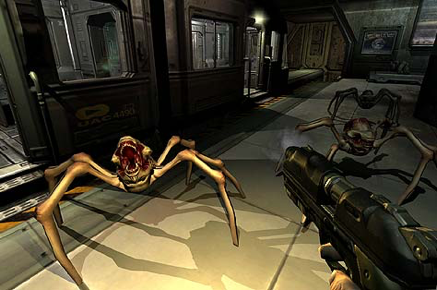
\includegraphics[height=3.6cm]{figs/pourtant1.png}
    \hspace{0.5cm}
    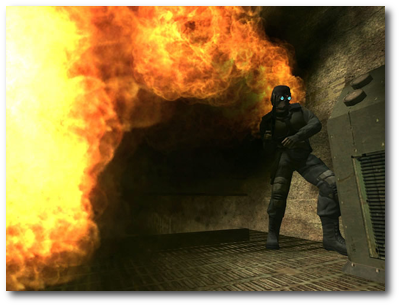
\includegraphics[height=3.6cm]{figs/pourtant2.png} \\
    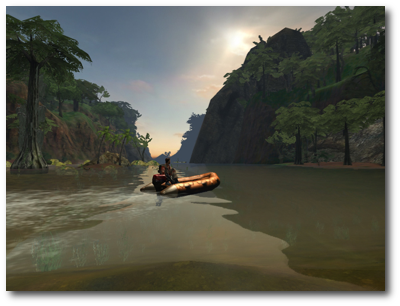
\includegraphics[height=3.6cm]{figs/pourtant3.png}
    \hspace{0.5cm}
    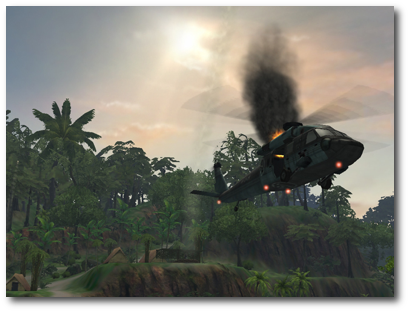
\includegraphics[height=3.6cm]{figs/pourtant4.png}
  \end{center}
\end{frame}
%--- Next Frame ---%

\begin{frame}[t]{Au delà des jeux vidéos : reflets simples}
  \begin{center}
    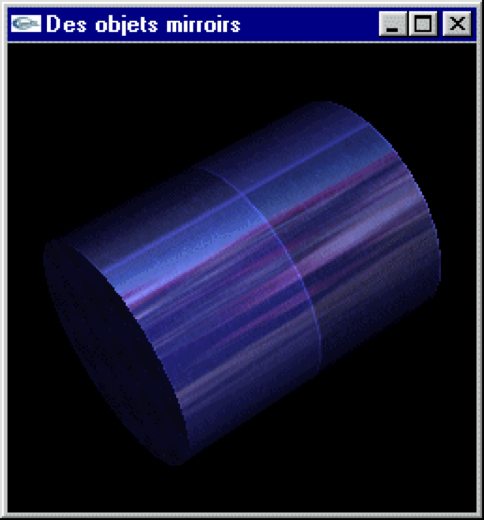
\includegraphics[height=4cm]{figs/reflets1.png}
    \hspace{0.5cm}
    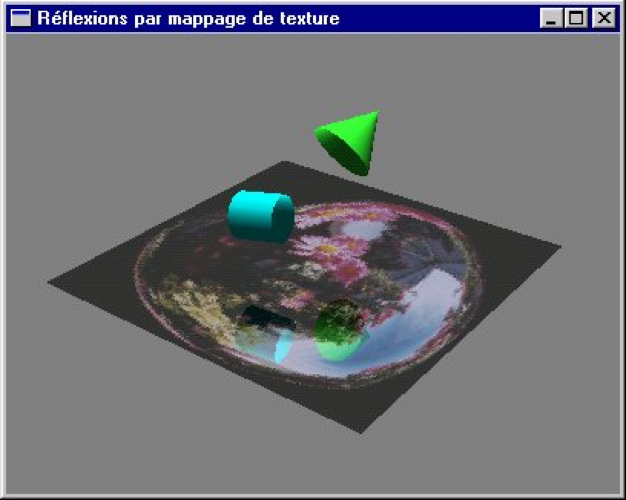
\includegraphics[height=4cm]{figs/reflets2.png}
  \end{center}
\end{frame}
%--- Next Frame ---%

\begin{frame}[t]{Au delà des jeux vidéos : ombres portées}
  \begin{center}
    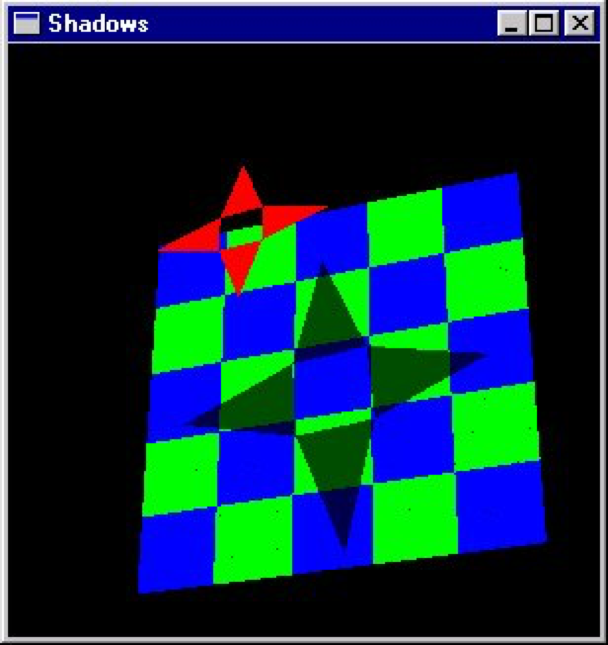
\includegraphics[height=4cm]{figs/shadow1.png}
  \end{center}
\end{frame}
%--- Next Frame ---%

\begin{frame}[t]{Au delà des jeux vidéos : motion blur}
  \begin{center}
    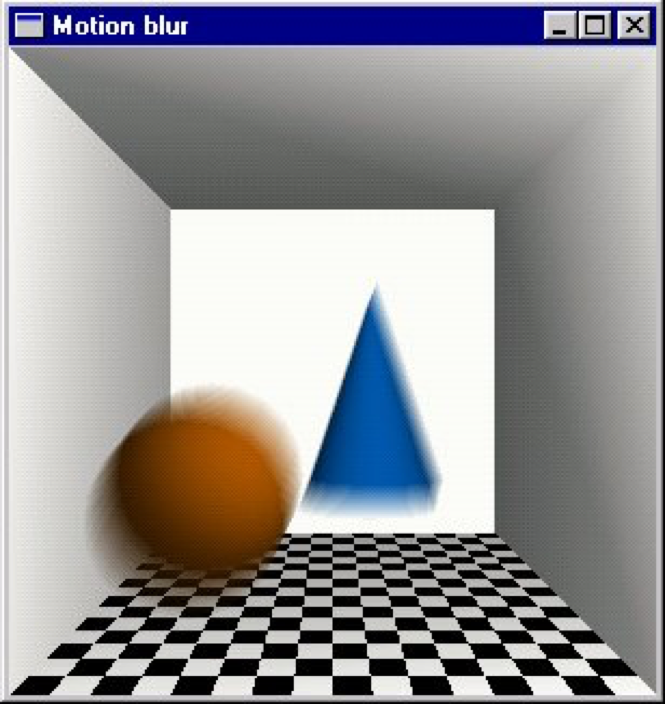
\includegraphics[height=4cm]{figs/motionblur.png}
  \end{center}
\end{frame}
%--- Next Frame ---%

\subsection{Interlude technique : ombres portées}

\begin{frame}[t]{Ombres portées en temps réel}
  \begin{itemize}

    \item Problème : déterminer les zones à l'ombre, i.e. celles qui ne sont pas visibles directement depuis la source lumineuse

    \item Principe
      \begin{itemize}
        \item réutiliser l'algorithme d'élimination des faces cachées \textbf{depuis l'origine de la source lumineuse}
        \item Trouver une technique de rendu des ombres (projection, polygones d'ombres...)
      \end{itemize}
    \item Coût : rendu en deux passes au lieu d'une
  \end{itemize}
  \begin{center}
    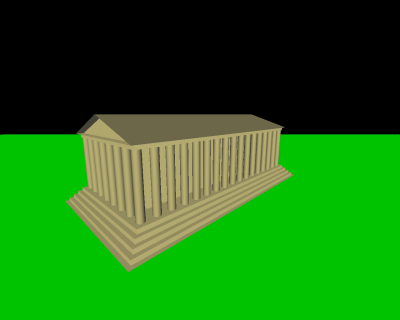
\includegraphics[height=1.7cm]{figs/3noshadow.png} \hspace{0.1cm}
    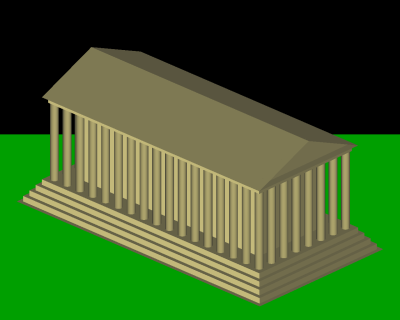
\includegraphics[height=1.7cm]{figs/1light.png} \hspace{0.1cm}
    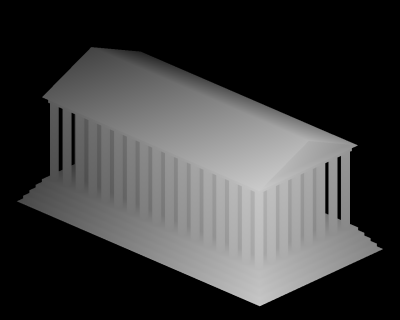
\includegraphics[height=1.7cm]{figs/2shadowmap.png} \hspace{0.1cm}
    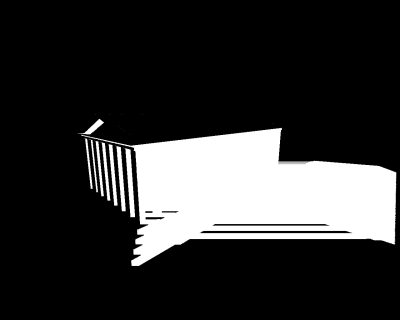
\includegraphics[height=1.7cm]{figs/5failed.png} \hspace{0.1cm}
    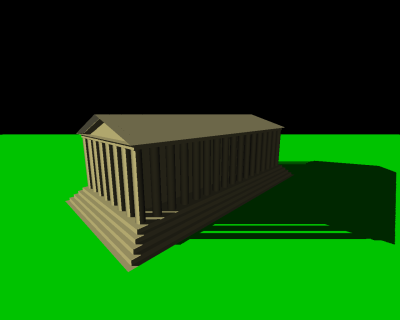
\includegraphics[height=1.7cm]{figs/7fin.png} \hspace{0.1cm}
  \end{center}
\end{frame}
%--- Next Frame ---%
